% !TeX root = ../main.tex

\xchapter{生成式EIT图像重建算法理论基础}{Theory of Generative EIT Reconstruction Algorithm}

EIT技术是一种根据场域边界电压信息重构场域内电导率分布信息的成像技术。该技术由
于其非侵入、无损伤等优势,近年来得到了广泛的应用。然而,EIT 图像重建算法由于其固
有的不足而限制了其使用场景。因此,如何提高重建图像的分辨率,并加快重建的速度,是
目前 EIT 技术的瓶颈。

近年来,深度学习技术,尤其是生成式模型,取得了突破性的成果,这也为提高 EIT 图
像重建质量提供了新的研究方向。不同于计算机视觉领域的其他图像生成任务(如利用文本
生成图像、图像分类、图像识别等),EIT 技术具有完备的数学物理模型,这就为基于深度学
习的 EIT 图像重建模型提供了大量的仿真数据支持。然而,由于其性能直接影响了临床医生
对于病情的判断,因此 EIT 图像重建算法的广泛应用需要确保其效率及可行性。

本章将主要介绍 EIT 图像重建算法的数学原理,深度学习和生成式模型的常见构件及模
型结构。随后将重点对两者之间结合的可行性以及优势作出阐述,为构建基于生成式模型的
EIT 图像重建算法提供理论基础。

\xsection{EIT基本原理}{Basic Principle of EIT}
\label{PrincipleEIT}
\xsubsection{EIT问题模型}{Model of EIT Problem}
在工程数学领域通常对事物内部的特征进行参数化,用模型参数$\boldsymbol{m}$来表示,它属于模型参数域$M$。
这些参数在工程实践中通常难以观测得到。
因此会选取一些与该模型参数有显著相关性的可观测参数$\boldsymbol{d}$来推断得到模型参数,
其中$\boldsymbol{d}$属于可测量参数域$D$。
则正问题可被描述为通过已知的模型参数$\boldsymbol{m}$求解可测量参数$\boldsymbol{d}$,即\cref{equation:forward}
\begin{equation}
  \label{equation:forward}
  \boldsymbol{d} = h(\boldsymbol{m})
\end{equation}
特别的,线性正问题可被描述为\cref{equation:linear_forward}
\begin{equation}
  \label{equation:linear_forward}
  \boldsymbol{d} = \boldsymbol{H}\boldsymbol{m}
\end{equation}
其中,$\boldsymbol{H}$为矩阵算子。
则逆问题则被描述为已知测量参数$\boldsymbol{d}$求解模型参数$\boldsymbol{m}$的过程。

然而,在实际的工程中,往往无法直接获得逆问题的精确解,或根本不可能获得唯一的精确解,
即不可能满足\cref{equation:error}这是由于实际问题中的每一步都存在一定的误差。
\begin{equation}
  \label{equation:error}
  h(\boldsymbol{m}) - \boldsymbol{d} = 0
\end{equation}

EIT技术通过向未知场内注入电流,同时测
量其边界电压分布,利用麦克斯韦方程组求解出其场域内部的电导率(或阻抗,注:由于电
导率和电阻抗之间为倒数关系,可相互转换。虽 EIT 名为电阻抗断层成像,但在实际 EIT 的
研究中,通常利用电导率分布作为重建图像的直接依据,故如无特殊说明,本文的成像目标
均为电导率)分布,最后根据其内部的电导率分布重建出图像(如\cref{figure:eeeee})。

\begin{figure}[h]
  
  \centering

\begin{tikzpicture}

  % 画圆
  \draw (0,0) circle (2cm);
  
  % 画16等分点
  \foreach \i in {1,...,16} {
      \draw (360/16*\i:2cm) circle (2pt);
  }
  
  % 标注电极
  \node at (360/16:2.5cm) {电极};
  
  % 标注注入电流箭头
  \draw[->] (90:2.5cm) -- (90:2cm) node[above]{\quad\quad\quad\quad\quad\quad 注入电流};
  % 标注出去的箭头
  \draw[->] (270:2cm) -- (270:2.5cm);
\end{tikzpicture}
\caption{待测场图示}
\label{figure:eeeee}

\end{figure}



EIT问题属于电磁场分析问题,其电导率分布、注入电流以及测量电压之间可根据麦克斯
韦(Maxwell)方程组建模。

\begin{equation}
\label{equation:Maxwell}
    \begin{aligned}
        \nabla \times \boldsymbol{H} &= J + \frac{\partial{D}}{\partial{t}} \\
        \nabla \cdot \boldsymbol{D} &= \rho \\
        \nabla \cdot \boldsymbol{B} &= 0 \\
        \nabla \times\boldsymbol{E} &= -\frac{\partial \boldsymbol{B}}{\partial t} \\   
    \end{aligned}
\end{equation}
其中,$\nabla$为矢量微分算子(泊松算子),$\boldsymbol{H}$ 为磁场强度,$\boldsymbol{J}$ 为电流密度,$\boldsymbol{D}$
为电位移,$\boldsymbol{E}$ 为电场强度,$\boldsymbol{B}$为磁通量密度, $t$为时间,$\rho$为区域内的电荷密度.
在各向同性的电磁场中,$\boldsymbol{J}$、$\boldsymbol{E}$、$\boldsymbol{B}$、$\boldsymbol{D}$、$\boldsymbol{H}$之间满足以下关系(介质的本构关系),
\begin{equation}
  \label{equation:Maxwell_relation}
  \begin{aligned}
    \boldsymbol{D} &= \varepsilon\boldsymbol{E}\\
    \boldsymbol{B} & = \mu\boldsymbol{E}\\
    \boldsymbol{J} & = \sigma\boldsymbol{E}\\
  \end{aligned}
\end{equation}
式中,$\varepsilon$是介电常数,$\mu$是介质的磁导率,$\sigma$是电导率。

为简化 EIT 问题的求解步骤,通常作以下假设:

1)EIT 敏感场可被看作是似稳场。即 EIT 场域内部任意一点的电流在激励信号的作用下同
  时产生相应的变化。也就是说可以忽其场域内介电常数和位移电流的影响。

2)EIT 场域内部不存在其他与外部激励信号频率相同的电流源。即场域内部不存在涡流效
  应,任意位置电流密度的散度为 0。

3)假设激励电流仅流经单排电极所在的平面。即研究二维 EIT 问题,以降低问题的复杂性,
  提高计算效率。
根据以上假设,EIT 模型还满足:
\begin{equation}
  \label{equation:Maxwell_hp}
  \nabla \cdot \boldsymbol{J} = 0
\end{equation}
而电场强度$\boldsymbol{E}$和电位$\phi$之间满足
\begin{equation}
  \label{equation:Maxwell_EP}
  \boldsymbol{E} = - \nabla \phi
\end{equation}
则由式\cref{equation:Maxwell}、\cref{equation:Maxwell_EP}、\cref{equation:Maxwell_hp}、\cref{equation:Maxwell_relation}
可得拉普拉斯方程:
\begin{equation}
  \nabla \cdot (\sigma\nabla\phi) = 0
\end{equation}
上式即为EIT敏感场的数学模型。

由此EIT模型可被描述为:
对于连续的已知平面$\Omega$上的EIT模型,其电压分布$u(x,y)$满足如下方程和边界条件:
\begin{equation}
  \begin{aligned}
  &\nabla \cdot (\sigma \nabla \phi) = 0, &(x, y)\in {\Omega} \\
  &\sigma\frac{\partial{u}}{\partial{v}} = \psi, &(x,y) \in {\partial{\Omega}} \\
  &\phi = \varphi, &(x,y)\in\partial{\Omega} \\
\end{aligned}
\end{equation}
其中,其内部电导率分布$\sigma(x,y) > 0$ ,边界电流密度$\psi(x,y)$,边界电压$\phi(x,y)$,边界电压$\varphi(x,y)$均是关于场域内部任意一点($x,y)$的函数。

EIT问题包含EIT正问题和EIT逆问题,EIT正问题为:
若给定$\sigma(x,y)$和$\psi(x,y)$,则可由方程组确定出$u(x,y)$,即诺伊曼边界值问题。
若给定$\sigma(x,y)$和$\rho(x,y)$,求解$u(x,y)$,则为迪利克雷边界值问题。

而实际EIT问题需要求解逆问题,即已知边界电压$\rho$和电流$\psi$求解电导率分布$\sigma(x,y)$。
电导率分布$\sigma(x,y)$确定了从可能的电流密度集合$\Psi$到和电压分布集合$\Phi$的映射。
\begin{equation}
  F_\sigma: \psi(x,y) \rightarrow \phi(x,y)
\end{equation}
EIT逆问题即是在已知 $F_{\sigma} = F_0$的条件下求解 $\sigma(x,y)$,使得
\begin{equation}
  F_{\sigma}(\psi) = F_{0}(\psi),  \forall \psi \in \Psi
\end{equation}


\xsubsection{EIT正问题}{Forward Problem of EIT}

EIT 正问题是指已知待测场内部的电导率分布及其边界电流驱动信号,求解其内部或边界的电压或
电流分布。
在实际求解中,通常求解出其解析解(精确解)非常困难,因此通常使用基于有限元的迭代方法求解出其近似解,EIT有限元模型如\cref{figure:FEMa}所示
\begin{figure}[h]
\centering
\includegraphics[width=.5\textwidth]{FEM.png}
\caption{有限元模型}
\label{figure:FEMa}
\end{figure}

则可设单元场域为\cref{figure:fem}所示,三角形单元各顶点$M_1(x_1,y_1)$,$M_2(x_2,y_2)$,$M_3(x_3,y_3)$的电位分别为
$\Phi_1$,$\Phi_2$,$\Phi_3$。用向量表示为:
\[
  \Phi =
  \begin{pmatrix}
  \Phi_1 \\
  \Phi_2 \\
  \Phi_3
  \end{pmatrix}
  \]
\begin{figure}[htbp]
    \centering
    
  \begin{tikzpicture}[scale=1.5]
   
   
    % 坐标轴
    \draw[->] (-1,0) -- (3,0) node[right] {$x$};
    \draw[->] (0,-1) -- (0,3) node[above] {$y$};
    
    % 三角形
    \coordinate (M1) at (2,1);
    \coordinate (M2) at (2.5,2.5);
    \coordinate (M3) at (1.5,2);
  
    \draw  (M1) node[right] {$M_1(x_1,y_1)$} -- (M2) node[above right] {$M_2(x_2,y_2)$} -- (M3) node[above left] {$M_3(x_3,y_3)$} -- cycle;
  
  \end{tikzpicture}
  \caption{三角形单元}
  \label{figure:fem}
\end{figure}
令三角形单元内部的电位分布为:
\begin{equation}
  \Phi(x,y) = \alpha + \beta x + \gamma y 
\end{equation}
进一步将三角形顶点的坐标和电位带入求解可得:
\begin{equation}
  \Phi_e(x,y) = \frac{\Phi_1}{2\Delta}(a_1+b_1x+c_1y) + \frac{\Phi_2}{2\Delta}(a_2+b_2x+c_2y) + \frac{\Phi_3}{2\Delta}(a_3+b_3x+c_3y)
\end{equation}
其中,
\begin{equation}
  \left\{
  \begin{array}{c}
    a_1 = x_2y_3 - x_3y_2 \\
    a_2 = x_3y_1 - x_1y_3 \\
    a_3 = x_1y_2 - x_2y_1
  \end{array}
  \right.
  \qquad 
  \left\{
    \begin{array}{c}
      b_1 = y_2 - y_3 \\
      b_2 = y_3 - y_1 \\
      b_3 = y_1 - y_2
    \end{array}
    \right.
    \qquad 
    \left\{
      \begin{array}{c}
        c_1 = x_3 - x_2 \\
        c_2 = x_1 - x_3 \\
        c_3 = x_2 - x_1
      \end{array}
      \right.
\end{equation}
$\Delta = b_1c_2 - b_2c_1$为三角形的面积。
进一步令:
\begin{equation}
  B = \frac{1}{2\Delta} \left[
  \begin{array}{ccc}
    b_1 & b_2 & b_3 \\
    c_1 & c_2 & c_3 \\
    
  \end{array}
  \right]
\end{equation}
可求得三角形内部泛函为:
\begin{equation}
  F_e(\Phi) = \frac{1}{2} \Phi K_e \Phi^T - \Phi Q_e
\end{equation}
其中,
根据每个点的坐标可分别求得单元刚度矩阵$K$中各元素的值:
\begin{equation}
  K = 
  \left[
  \begin{array}{ccc}
    \frac{b_1^2 + c_1^2}{4\Delta \rho} & \frac{b_1b_2 + c_1c_2}{4\Delta \rho} & \frac{b_1b_3 + c_1c_3}{4\Delta \rho}  \\
    \frac{b_1b_2 + c_1c_2}{4\Delta \rho} & \frac{b_2^2 + c_2^2}{4\Delta \rho} & \frac{b_2b_3 + c_2c_3}{4\Delta \rho} \\
    \frac{b_1b_3 + c_1c_3}{4\Delta \rho} &  \frac{b_2b_3 + c_2c_3}{4\Delta \rho}& \frac{b_3^2 + c_3^2}{4\Delta \rho} 
  \end{array}
  \right]
\end{equation}
则待测场内总体泛函为
\boldmath
\begin{equation}
  F_e(\Phi) = \frac{1}{2} \Phi K \Phi^T - \Phi Q_e
\end{equation}
\unboldmath
进一步,对泛函取极值,得到线性方程组:
\boldmath
\begin{equation}
  K\Phi = Q
\end{equation}
\unboldmath
其中K为总体刚度矩阵,由单元刚度矩阵叠加而成\cite{2019d_cc}。由此可见,EIT正问题求解,主要通过变分法代替原问题,后将问题离散化一般的极值问题。
其对于边界形状任意变化的待测场也适用。也正是EIT正问题完备的仿真模型给利用深度学习模型实现EIT图像重建算法提供了数据基础。

\xsubsection{EIT逆问题}{Inverse Problem of EIT}
EIT 逆问题是指已知场域边界的测量电压以及驱动信号,求解场域内部的电导
率分布情况,其在理论上存在唯一解已被先前的研究证实\cite{Sun1993An}。其条件则是已知$\rho(x,y),\quad x \in \partial \Omega$。
然而对于实际的工程问题而言,对于一个未知场,其可获得的边界电压值是有限的,即电极的个数限制了测量数据的维度。
这就导致EIT逆问题的严重病态性以及非适定性,进而影响了重建分辨率。
EIT逆问题的求解往往通过迭代的思想,根据每一步正问题求解后边界电压与真实测量结果的误差不断修正系统参数。
因此实现高质量EIT图像重建算法的关键即优化EIT逆问题求解的过程。

\xsection{深度学习相关理论}{Theory of Deep Learning}
近年来深度学习技术发展迅速,各种架构层出不穷,而本文所提出的EIT图像重建算法以深度学习模型为基础,因此本章将重点介绍该算法中所用到的深度学习技术的原理和架构。
\xsubsection{全连接神经网络}{Fully Connected Neural Networks}
全连接神经网络(Fully Connected Neural Networks, FCN),也被称为人工神经元网络(Artificial Neural Network,ANN),多层感知机(Multilayer Perceptron,MLP)。
该思想源于仿生学,其中树突对应MLP的输入层,轴突和轴突未梢对应其隐藏层和输出层。
FCN是深度学习模型中最基础的结构。一个三层的MLP包含了其模型如\cref{figure:FCN}所示,每层神经元本质上代表一组权重矩阵,用来对输入层的数据做线性变换(或仿射变换),进而输出至下一层。
通常,输出层的数据会通过一个激活函数后输出最终结果。每层神经元的输出是下一层所有神经元的输入,故名“全连接”。
全连接网络有对非线性映射强大的拟合能力,故可以用来学习各种非线性映射。然而,随着神经网络层数的增加,其训练和推理过程由于网络参数规模庞大而往往更加耗时。
同时,全连接网络的输入通常为向量,因此会忽略掉二维或高维数据的空间特征。因此,当前主流的深度学习模型通常不以FCN作为主要模型架构,取而代之的是卷积神经网络等,以更好地适应复杂的任务和高维的数据。
FCN更多地是用作一个模型的一小部分。
\begin{figure}[H]
  \usetikzlibrary{positioning}
  

  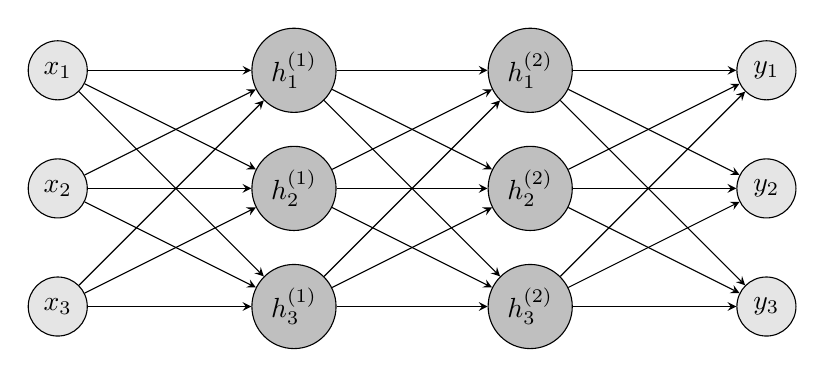
\begin{tikzpicture}[x=1.5cm, y=1.5cm, >=stealth]
  
  % 输入层
  \foreach \m/\l [count=\y] in {1,2,3}
      \node [circle,draw,fill=gray!20,minimum size=0.75cm] (input-\m) at (0,2.5-\y) {$x_\l$};
  
  % 隐藏层
  \foreach \m [count=\y] in {1,2,3}
      \node [circle,draw,fill=gray!50,minimum size=0.75cm] (hidden1-\m) at (2,2.5-\y) {$h_\m^{(1)}$};
  \foreach \m [count=\y] in {1,2,3}
      \node [circle,draw,fill=gray!50,minimum size=0.75cm] (hidden2-\m) at (4,2.5-\y) {$h_\m^{(2)}$};
  
  % 输出层
  \foreach \m [count=\y] in {1,2,3}
      \node [circle,draw,fill=gray!20,minimum size=0.75cm] (output-\m) at (6,2.5-\y) {$y_\m$};
  
  % 连接
  \foreach \m in {1,...,3}
      \foreach \n in {1,...,3}
          \draw [->] (input-\m) -- (hidden1-\n);
  \foreach \m in {1,...,3}
      \foreach \n in {1,...,3}
          \draw [->] (hidden1-\m) -- (hidden2-\n);
  \foreach \m in {1,...,3}
      \foreach \n in {1,...,3}
          \draw [->] (hidden2-\m) -- (output-\n);
  
  \end{tikzpicture}
  \caption{全连接神经网络}
  \label{figure:FCN}
\end{figure}

\xsubsection{卷积神经网络}{Convolutional Neural Networks}
卷积神经网络(Convolutional Neural Networks, CNN)是目前使用范围最广的深度学习模型之一,由其对高维数据的空间特征提取能力的优异表现而广泛应用于图像处理和计算机视觉任务中。
一般的CNN通常包含卷积层,池化层,全连接层。其常见的模型结构如\cref{figure:CNN}所示。

\begin{figure}[h]
  \centering
\includegraphics[width=0.6\textwidth]{CNN.JPG}
\caption{卷积神经网络结构示意}
\label{figure:CNN}
\end{figure}

卷积层通常利用卷积操作提取图像(或其他输入数据)的空间特征信息。CNN每一层通常具有多个通道(包含多个卷积核),每个卷积核分别与图像进行卷积运算,其的结果将会作为下一层的输入;不同的卷积核可以提取到图像不同类型的空间特征,因此CNN通常相较于FCN有更强大的特征提取能力。
池化层通常用于减小图像尺寸,同时可以保留输入结果中重要的特征信息。常见的池化操作通常有平均值池化(Average Pool)、最大值池化(Max Pool)等。
全连接层则是将CNN的输出结果进行重塑,使得输出维度符合实际需要。通常用于分类或回归预测等任务中。
CNN的运算原理如\cref{equation:CNN}所示。
\begin{equation}
  \label{equation:CNN}
  Y = \sigma\left(\sum_{i=1}^{n} \boldsymbol{W_i} conv(\boldsymbol{X_i}) + \boldsymbol{b}\right)
\end{equation}

其中:
$\mathbf{Y}$ 是输出特征图;
$\sigma(\cdot)$ 是激活函数;
$n$ 是卷积核的数量;
$\mathbf{W}_i$ 是第 $i$ 个卷积核的权重;
$\mathbf{X}_i$ 是与第 $i$ 个卷积核进行卷积的输入特征图;
$\mathbf{b}$ 是偏置项;
$conv(\cdot)$ 表示卷积操作。
自Resnet提出以来\cite{2016Resnet},残差卷积以广泛应用在各种基于卷积神经网络的模型之中其核心思想是通过残差连接来解决神经网络中的梯度消失以及梯度爆炸问题。其模型如\cref{figure:Resnet}
通常这种结构可以使得网络直接学习残差(即残差块的输出减去输入)。本文大量采用了残差卷积块作为模型的基础模块,这种方式可以使整个网络更容易优化和训练,进一步提高网络的性能和泛化能力。
\begin{figure}[h]
  \centering
  \includegraphics[width=0.6\textwidth]{Resnet.png}
  \caption{残差卷积模型}
  \label{figure:Resnet}
\end{figure}



\xsubsection{激活函数}{Activation Functions}

神经网络在各个领域的广泛应用主要得益于其对于非线性映射的强大拟合能力,
这种拟合能力,主要来自于非线性激活函数。
而深度学习模型如CNN,FCN等基础模块的运算通常为大量的线性映射(加法和乘法)。
因此,选择适当的激活函数,对于深度学习模型性能的提升将是显著的。
近年来,各式各样的激活函数不断被学者们提出,本文将重点介绍模型从采用的四种激活函数,如
对于其他未被使用到的激活函数将不做赘述。


\subsubsection{ReLU}

ReLU是Hinton于2010年提出的激活函数\cite{2010ReLU},其表达式如\cref{equation:ReLU}所示。
sigmoid函数在函数值趋近于0和1的时候会变得平坦,即此时的梯度几乎为0。而由于神经网络参数更新的方式通过反向传播进行,则此时对于这类输入或输出趋于0的节点,其权重几乎不会得到更新,此类神经元被称为饱和神经元。
因此,这就会导致神经网络中许多节点的参数不再更新,即梯度消失问题。
ReLU在输入大于0的时候其梯度恒为1,因此可以有效避免梯度消失问题,并且由于其中只存在线性映射,因此能大大提高网络的计算效率,进而加快梯度下降过程中的收敛速度。
此外,该激活函数还被认为具有生物和理性,即与单侧抑制原理相符。

  \begin{equation}
    \label{equation:ReLU}
    \sigma(x) = 
    \left\{
    \begin{aligned}
      0, \quad x <= 0 \\
      x, \quad x > 0
    \end{aligned}
    \right.
    \end{equation}

    \subsubsection{SiLU}
  
    SiLU的表达式如\cref{equation:SiLU}所示。
    其相较于ReLU而言,由于其连续可微,故在反向传播的过程中更容易优化。并且SiLU在其定义域内梯度均不为0,这非常有助于在深度神经网络中避免梯度消失的问题。
    同时,由于ReLU函数的特性,网络中输出结果小于0的神经元会被抑制(其梯度为0),故会造成网络稀疏,虽然有助于抑制过拟合,但是也会抑制网络对于数据信息的利用率,进而影响模型的性能。
    并且由于ReLU和Sigmoid函数的输出数据分布的均值均不为零,因此会给后一层的神经网络引入偏置偏移,进而可能会影响梯度下降的效率。
    而,SiLU的输出范围在$[0, 1]$之间,因此可以为后续的模块保留一定的动态范围,从而有助于更好地处理数据分布的变化。

    \begin{equation}
      \label{equation:SiLU}
      \text{SiLU}(x) = x \cdot \sigma(x)
    \end{equation}
  其中,$\sigma(x)$ 是 Sigmoid 函数,定义为:
  \begin{equation}
    \sigma(x) = \frac{1}{1 + e^{-x}}
  \end{equation}
  
  \subsubsection{Gaussian Error Linear Units function (GeLU)}
  
  GeLU是2016年 Hendrycks等人提出的激活函数\cite{2016GeLU}。但直到其在Transformer和Bert模型中得到应用之后,才广泛进入人们的视野。
  该函数的表达式如\cref{equation:GeLU}。
  其中,$\Phi(x)$ 是标准正态分布的累积分布函数(CDF),可以用高斯误差函数(erf)的形式表示。
  GeLU函数通过给输入向量乘以一个权重,该权重是输入变量的非线性映射(即高斯误差函数),其原理与ReLU和Dropout类似。
  不同的是,ReLU会为输入向量乘以固定的权重1(或0),而dropout则会为部分输入乘以0(即抛弃该输入)。
  GeLU所乘的系数,这是与输入变量的自身分布有关。由此,GeLU可以将输入变量$x$平滑地映射到高斯分布的CDF上。
  重要的是,GeLU在最近的深度学习模型中通常表现出优于ReLU或ELU等传统的激活函数。

  \begin{equation}
    \label{equation:GeLU}
    \text{GELU}(x) = x \cdot \Phi(x) 
  \end{equation}
   \begin{equation}
    \label{equation:Gauss}
    \Phi(x) = \frac{1}{2} \left(1 + \text{erf} \left(\frac{x}{\sqrt{2}}\right)\right)
  \end{equation}
  

  \subsubsection{Softmax}

  Softmax函数不同于其他激活函数,其作用是将连续的输出信号映射到离散的空间中,故经常用作分类网络的输出层,其计算方式如\cref{equation:softmax}所示。
  Softmax计算该层每个神经元的输出对所有神经元输出的和的比值。即此过程将每个神经元的输出映射到了$[0,1]$中,并且输出层
  所有的神经元之和为1。这样做的好处则是输出层的神经元可以表示为一个概率空间,其中每个神经元的输出可以看做是某一个事件发生的概率。
  因此经常作为多分类问题的输出层使用。

\begin{equation}
  \label{equation:softmax}
  \text{softmax}(\mathbf{z})_i = \frac{e^{z_i}}{\sum_{j=1}^{K} e^{z_j}}
\end{equation}

其中,$\mathbf{z} = (z_1, z_2, ..., z_K)$ 是输入向量,$K$ 是类别的数量。softmax 函数将输入向量的每个元素 $z_i$ 转换为相应的概率值,即满足所有概率之和等于1。



\begin{figure}[h]
  \centering
\includegraphics[width=0.7\textwidth]{activation.png}
\caption{激活函数}
\label{figure:activation}
  
\end{figure}



\xsubsection{优化器}{optimizer}
大多数神经网络的参数更新是通过反向传播算法实现的,其利用损失函数计算输出层的结果与真实的标签数据分布之间的误差,称为网络输出层的损失(loss),然后根据链式法则求出该损失对每一层神经元的参数的损失,然后利用这些损失对网络中每一个参数分别更新。
其中优化器的选择通常决定了如何利用损失函数更新网络参数。

最基础且常见的优化器即为随机梯度下降法(Stochastic Gradient Descent,SGD),在网络模型中的参数初始化之后,该方法首先在训练集中随机选择一个样本,用作本轮计算损失的数据。
然后再利用所选择的损失函数(通常为均方误差损失函数或交叉熵损失函数)计算出输出结果与真实标签分布之间的损失,并利用反向传播算法求出每一步用于更新参数的损失,最后利用\cref{equation:SGD}更新网络参数。

\begin{equation}
  \label{equation:SGD}
  \theta_{t+1} = \theta_{t} - \eta \nabla J(\theta_{t}, x_i, y_i)
\end{equation}
其中,$\theta_{t}$表示第$t$次迭代时模型中的所有参数集,其中包含所有可学习的参数如网络权重等。
$\eta$是学习率(learning rate),用于控制每一步参数更新的步长
$\nabla J(\theta_{t}, x_i, y_i)$则表示损失函数$J$对参数 $\theta_{t}$在样本$i$上的梯度 ;
而$x_i$、$y_i$分别是样本的特征向量(原始数据集中的样本)和样本的标签(label)。
由于随机梯度下降法通常只选择一个样本用来计算梯度,因此训练时间较短,并且训练的方向具有一定的随机性,通常可以跳出局部最优解,从而在更广泛的参数空间中优化网络参数。

但也正是因为其梯度更新方向的随机性,SGD对网络参数更新的频率通常较高,收敛速度可能较慢,并且波动较大,从而导致参数更新不够稳定。

传统的如各种梯度下优化算法通常会将学习率设置为固定值,或硬编码其学习率(如让其成为epoch的函数),这样做就忽略了学习率其他变化的可能性。
因此就产生了自适应学习率优化算法如Adaptive Gradient(AdaGrad)、RMSProp和Adaptive Moment Estimation(Adam)等。

本文在网络模型训练的过程中大量使用了Adam优化算法\cite{2014Adam},这是因为该优化算法通过引入动量项,从而使其具有自适应的学习率(能够根据参数的梯度自动设置学习率,并且该学习率通常有一个固定的范围,这就一定程度上提高了模型参数的稳定性,从而提高了模型收敛的速度,加快了训练过程)。
Adam结合了Adagrad和RMSprop算法的优点,使得其算法更加善于处理稀疏梯度和非平稳目标。
此外也可被用在非凸优化任务中,即适用于大规模的数据集并应用在高维的参数空间中。
Adam优化器在网络模型参数初始化后,还要初始化优化器的超参数,默认$\beta_1 = 0.9$,$\beta_2 = 0.999$控制动量的指数和衰减率;$\epsilon = 10^{-8}$用于防止分母为零,学习率$\eta = 0.001$。
其迭代式如\crefrange{equation:Adamiter:a1}{equation:Adamiter:a5}所示。
\begin{equation}
  \label{equation:Adamiter:a1}
  \centering
  m_t  = \beta_1 m_{t-1} + (1 - \beta_1) g_t
\end{equation}
\begin{equation}
  \label{equation:Adamiter:a2}
  \centering
  v_t  = \beta_2 v_{t-1} + (1 - \beta_2) g_t^2
\end{equation}
\begin{equation}
  \label{equation:Adamiter:a3}
  \centering  
  \hat{m}_t  = \frac{m_t}{1 - \beta_1^t}
\end{equation}
\begin{equation}
  \label{equation:Adamiter:a4}
  \centering
  \hat{v}_t  = \frac{v_t}{1 - \beta_2^t} 
\end{equation}
\begin{equation}
  \label{equation:Adamiter:a5}
  \centering
  \Delta \theta_t  = -\frac{\eta}{\sqrt{\hat{v}_t} + \epsilon} \hat{m}_t 
\end{equation}
\begin{equation}
  \label{equation:Adamiter:a6}
  \theta_{t+1} = \theta_t + \Delta \theta_t 
\end{equation}
其中,$m_t, v_t$分别表示一阶和二阶动量,$\hat{m}_t, \hat{v}_t$分别表示对一阶以及二阶动量校正偏差后的值的估计。
$\Delta\theta_t$ 表示每部参数更新的量,$\theta_t$表示第$t$步中网络参数值。

\xsection{生成式模型}{Generative Models}
EIT图像重建算法的任务目标即是在给定边界条件下生成出符合原始电导率分布的图像。
通常基于深度学习模型设计的EIT图像重建算法利用电压-电导率分布数据构件数据集,学习出电压到电导率分布的非线性映射以实现对EIT待测场中的目标信息进行成像。
此类深度学习模型的目标是估计$p(C \mid v)$(在已有的观测数据分布上估计目标变量的概率分布),其中$C$是电导率分布的真实概率分布,$v$是测量电压构成的向量组。
而实际情况下很难拟合出上述复杂的概率分布模型,故深度学习模型通常有两类不同的做法,即判别式模型和生成式模型。

判别式模型如卷积神经网络等通常通以$P(C \mid V=v)$为目标,即拟合$f(v) = p(c \mid v)$这一非线性映射。
不同于判别式模型,生成式模型则是先估计出$p(v \mid c)$ 再通过贝叶斯公式(\cref{equation:bysf})计算出$p(c \mid v)$。
\begin{equation}
  \centering
  \label{equation:bysf}
  p(c \mid v) = \frac{p(c, v)}{p(v)} = \frac{p(v \mid c)p(c)}{p(v)} 
\end{equation}

故生成式模型的本质是建立一个映射$X=g(Z)$,从隐变量的分布(latent variable)$Z$生成数据的真实分布。通常假设隐变量的分布为高斯分布(Gaussian Distribution)。
生成式模型的学习目标即通过一组数据($\mbs{X} = \{X_1, X_2, ..., X_i\}, i = 1, 2, ..., n$)学习其真实分布$p(X)$。即假设该数据集是从一个概率分布$p(x)$中采样的结果,生成式模型希望根据该采样结果(即数据集)恢复出这个概率分布。此后通过采样即可生成符合此分布的数据。
而由于恢复该分布较为困难,因此根据贝叶斯公式,在此过程中引入隐变量$Z$,利用隐变量$Z$与原始数据的关系计算出原始数据的概率分布$p(x)$,如\cref{equation:GenerativeModel}(离散情况),\cref{equation:GenerativeModelcon}(连续情况)。

\begin{equation}
  \centering
  \label{equation:GenerativeModel}
  P(x) = \sum_{Z}^{}p(x\mid Z)p(Z)
\end{equation}

\begin{equation}
  \centering
  \label{equation:GenerativeModelcon}
  p(x) = \int_{z \in Z}^{} p(x|z)p(z)\diff z
\end{equation}

变分自编码器(Variational Auto Encoder, VAE)就是生成式模型的一种,如\cref{figure:VAE}所示。其编码器将原始的数据分布$\mathbb{R}^n$映射到隐变量空间$\mathbb{R}^d$中,其隐变量空间为一组高斯分布的均值和方差。
\begin{figure}[h]
  \centering
  \includegraphics[width=.7\textwidth]{VAE.png}
  \caption{VAE架构}
  \label{figure:VAE}
  \end{figure}

即该编码器需要通过已知的观测样本$\mbs{X}$,计算出$p(z|x)$,如式\cref{equation:bysVAE}。

\begin{equation}
  \centering
  \label{equation:bysVAE}
  p(z \mid x) = \frac{p(x \mid z)p(z)}{p(x)} 
\end{equation}

然而,由于无法事先确定数据集采样的源分布$p(x)$,因此VAE通过利用一个可控制的分布$q(z|x)$来近似估计$p(z|x)$。
而由于K-L散度(Kullback-Leibler divergence,)可以很好地度量两个概率分布$P$和$q$之间的差异(该度量为非对称性的,如\cref{equation:KLdivergence}),

\begin{equation}
  \centering
  \label{equation:KLdivergence}
  D_{\text{KL}}(P \| Q) = \int_{x} P(x) \log \left( \frac{P(x)}{Q(x)} \right)
\end{equation}
故VAE的本质即最小化$p(z|x)$和$q(z|x)$的K-L散度(如\cref{equation:VAEKL})。
\begin{equation}
  \centering
  \label{equation:VAEKL}
  \min D_{\text{KL}}(q(z|x)\|p(z|x)) = \int_{x}q(z|x)\log \frac{q(z|x)}{p(z|x)}\diff Z
\end{equation}
上式经过计算可等价为\cref{equation:KLeq},
\begin{equation}
  \centering
  \max  \mathbb{E}_{z\sim q(z|x)} \log p(x|z) - D_{\text{KL}}(q(z|x)\|p(z))
  \label{equation:KLeq}
\end{equation}
即,最大化在$z$上采样的结果经过VAE后输出的重构结果为$x$的概率(等价于最小化网络输出结果与真实数据之间的均方误差),且让$q(z|x)$和$p(z)$尽可能相似。


除了VAE之外,Jonathan Ho等人提出的去噪的扩散概率模型\cite{DDPM}(Denoising Diffusion Probabilistic Models, DDPM)如\cref{figure:DDPM}以及后续的各种变体如条件扩散模型\cite{CondDDPM}(Conditional Denoising Diffusion Probabilistic Models),稳定扩散\cite{StableDiffusion}(Stable Diffusion)等已在图像生成领域取得了显著的成绩。
扩散模型的思想源于非平衡统计物理,其通过迭代完成正向的扩散过程从而系统、缓慢地破坏数据的结构。此后利用深度学习模型学习逆扩散的过程,从而恢复数据中的结构。由此产生了一个高度灵活且易于处理的数据生成模型。
其中,扩散的迭代次数通常可设定为千次左右。
\begin{figure}[h]
  \centering
  \includegraphics[width=.7\textwidth]{DDPM.jpg}
  \caption{DDPM原理}
  \label{figure:DDPM}
  \end{figure}

该模型同样是一个隐变量模型,即$p_\theta(x_o) \coloneqq \int p_\theta(x_{0:T})\diff x_{1:T}$,其中$x_1,...x_T$为隐变量,其大小和输入的$x_0$相同。
DDPM共包含两个主要部分,即正向扩散部分和逆向数据恢复部分。其中,通过不断添加高斯噪声使得原始数据映射到各向同性的高斯分布的过程称为扩散过程。在该过程中,原始的数据分布将随着时间逐渐扩散,并且不断接近高斯分布。
而将高斯分布通过加权的方式去噪声的过程通常称为逆扩散过程。两个过程均可看作是一个参数化的马尔科夫链(Markov Chain)。
因此,只需要训练一个用于生成每一步逆扩散过程中用于去噪声的网络,即可实现对于原始数据分布的拟合。


\xsubsection{小结}{Summary}
本章首先介绍了EIT技术的基本原理、传统EIT图像重建算法的实现过程以及其弊端。
随后介绍了常见的深度学习模型以及本文所使用到的深度学习相关技术。
最后介绍了实现本文所提出的EIT图像重建算法所用到的生成式模型,主要包括VAE的架构和扩散模型的基本原理。
为后续实现图像重建算法提供了理论基础。
